\documentclass[conference]{IEEEtran}
\IEEEoverridecommandlockouts
% The preceding line is only needed to identify funding in the first footnote. If that is unneeded, please comment it out.
\usepackage[T1]{fontenc}
\usepackage{cite}
\usepackage{mathtools}
\usepackage{stackengine}
\def\delequal{\mathrel{\ensurestackMath{\stackon[1pt]{=}{\scriptstyle\Delta}}}}
\usepackage{amsmath,amssymb,amsfonts}
\usepackage{amsmath,epsfig,cite,amsfonts,amssymb,psfrag,subfig}
\usepackage{graphicx}
\usepackage{textcomp}
\usepackage{xcolor}
\usepackage{algorithm}
\usepackage[noend]{algpseudocode}
\usepackage{amsthm}
\def\BibTeX{{\rm B\kern-.05em{\sc i\kern-.025em b}\kern-.08em
    T\kern-.1667em\lower.7ex\hbox{E}\kern-.125emX}}
\allowdisplaybreaks
\newtheorem{remark}{Remark}
\newtheorem{theorem}{Theorem}
\newtheorem{lemma}{Lemma}
\newtheorem{proposition}{Proposition}
\newtheorem{corollary}{Corollary}
\newcommand{\diag}{\mathop{\mathrm{diag}}}
\DeclareMathOperator{\E}{\mathbb{E}}
\usepackage[margin=0.7in]{geometry}
\setlength{\columnsep}{11mm}
\begin{document}

\title{Joint Power Allocation and Network Slicing in an Open RAN System \vspace{-.1cm}
}
%
%\author{\IEEEauthorblockN{1\textsuperscript{st} Mojdeh Karbalaee Motalleb}
%\IEEEauthorblockA{\textit{Electrical and Computer Engineering} \\
%\textit{Tehran University}\\
%Tehran, Iran \\
%mojdeh.karbalaee@ut.ac.ir}
%\and
%\IEEEauthorblockN{2\textsuperscript{nd} Vahid Shah-Mansouri}
%\IEEEauthorblockA{\textit{Electrical and Computer Engineering} \\
%\textit{Tehran University}\\
%Tehran, Iran \\
%vmansouri@ut.ac.ir}
%\and
%\IEEEauthorblockN{3\textsuperscript{rd} Salar Nouri Naghadeh}
%\IEEEauthorblockA{\textit{Electrical and Computer Engineering} \\
%\textit{Tehran University}\\
%Tehran, Iran \\
%salar.nouri@ut.ac.ir}
%}
  \author{
    \IEEEauthorblockN{Mojdeh Karbalaee Motalleb}
    \IEEEauthorblockA{School of ECE, College of Engineering, University of Tehran, Iran \\
    Email: \{mojdeh.karbalaee\}@ut.ac.ir,
    \vspace{-.2cm}
  }
  }

\maketitle

\begin{abstract}

\end{abstract}
\begin{IEEEkeywords}

\end{IEEEkeywords}
\section{Questions}
\begin{enumerate}
\item \textbf{Why deep Q learning is better than Q learning?}


Deep RL uses a Deep Neural Network to approximate Q(s,a). Non-Deep RL defines Q(s,a) using a tabular function.

Popular Reinforcement Learning algorithms use functions Q(s,a) or V(s) to estimate the Return (sum of discounted rewards). The function can be defined by a tabular mapping of discrete inputs and outputs. However, this is limiting for continuous states or an infinite/large number of states. A more generalized approach is necessary for large number of states.

Function approximation is used for a large state space. A popular function approximation method is Neural Networks. You can make a Deep Neural Network by adding many hidden layers.

Thus, Deep Reinforcement Learning uses Function Approximation, as opposed to tabular functions. Specifically DRL uses Deep Neural Networks to approximate Q or V (or even A).

When the environment gets complicated, the knowledge space can become huge and it no longer becomes feasible to store all (state, action) pairs. If you think about it in raw terms, even a slightly different state is still a distinct state (e.g. different position of the enemy coming through the same corridor). You could use something that can generalize the knowledge instead of storing and looking up every little distinct state.

So, what you can do is create a neural network, that e.g. predicts the reward for an input (state, action) (or pick the best action given a state, however you like to look at it)
So, what you effectively have is a NN that predicts the Q value, based on the input (state, action). This is way more tractable than storing every possible value like we did in the table above.

$Q = neural-network.predict(state, action)$
\begin{figure}%[H]
  \centering
    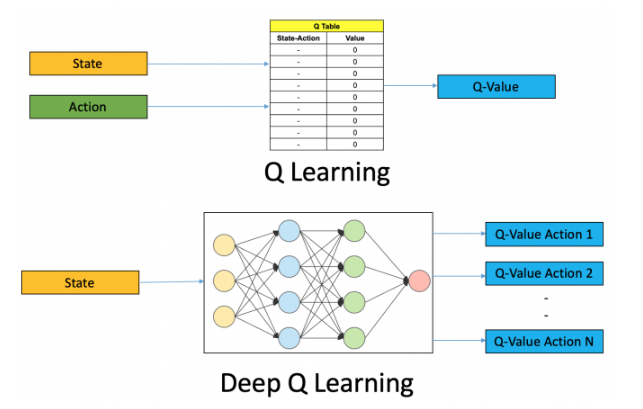
\includegraphics[width=\linewidth]{deepQ}
  \caption{deep Q learning structure \cite{drl}}
  \label{fig:drl}
\end{figure}
\item  \textbf{Find QoS that is required for different applications }
\begin{itemize}
\item \textbf{Bandwidth and throughput}: Bandwidth is the available capacity of connection between two terminals as the most popular term for that is (bps). Throughput slightly differs
from bandwidth as it stands for effective bandwidth that is
provided by network
\item \textbf{Delay or latency:} It specifies the time it takes for a packet
to leave source until reaching the destination. Applications
and network devices can cause delay.
\item \textbf{Jitter (delay variation):} Jitter is an interval between
subsequent packets. It is occurred by network congestion,
route alternation and etc. 
\item \textbf{Loss:} It is amount of packets out of all that are not received
at destination. The success of QOS depends on this factor.
\item \textbf{Reliability:} Some applications are sensitive to packet loss
such as real-time applications. Thus there must be some
mechanism either in application or network to minimize the
packet loss, such as forward error correction (FEC).
\end{itemize}
\begin{figure}%[H]
  \centering
    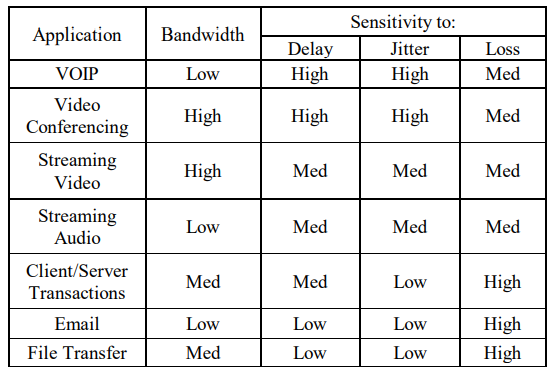
\includegraphics[width=\linewidth]{qos}
  \caption{deep Q learning structure \cite{qos}}
  \label{fig:qos}
\end{figure}
\item \textbf{Where do we use out of order delivery?}

out-of-order delivery is the delivery of data packets in a different order from which they were sent. Out-of-order delivery can be caused by packets following multiple paths through a network, or via parallel processing paths within network equipment that are not designed to ensure that packet ordering is preserved. One of the functions of TCP is to prevent the out-of-order delivery of data, either by reassembling packets into order or forcing retries of out-of-order packets.

Some applications running on your network are sensitive to delay. These applications commonly use the UDP protocol as opposed to the TCP protocol. The key difference between TCP and UDP as it relates to time sensitivity is that TCP will retransmit packets that are lost in transit while UDP does not. For a file transfer from one PC to the next, TCP should be used because if any packets are lost, malformed or arrive out of order, the TCP protocol can retransmit and reorder the packets to recreate the file on the destination PC.
\item \textbf{ What is the best method for online learning?! Game theory vs RL vs DRL vs Deep learning?}

In Reinforcement Learning (RL) it is common to imagine an underlying Markov Decision Process (MDP). Then the goal of RL is to learn a good policy for the MDP, which is often only partially specified. MDPs can have different objectives such as total, average, or discounted reward, where discounted reward is the most common assumption for RL. There are well-studied extensions of MDPs to two-player (i.e., game) settings.

Game theory is quite involved in the context of Multi-agent Reinforcement learning (MARL).

RL: A single agent is trained to solve a Markov decision problem (MDPS). GT: Two agents are trained to solve Games. A multi-agent Reinforcement learning (MARL) can be used to solve for stochastic games.

If you are interested in the single-agent application of RL in deep learning, then you do not need to go for any GT course. For two or more agents you may need to know the game-theoretic techniques.

So a big differences is that mostly RL is a single agent decision and GT is a multiple agent decision.

Then there are minor differences related to the most common uses. RL uses decision through time, GT only equilibria points. RL considers infinite state space, GT considers finite ones. RL is a learning problem (you have to learn the model of the world) while GT is a planning problem (you already know your game matrix). Of course there are exception to all these minor differences.

For instance it is easy to prove that two agents using Q-Learning in a competitive game will converge to the Nash equilibria of a game.
%%
The reinforcement learning techniques enable a single
agent to learn optimal behavior through trial-and-error interactions with its environment. Various RL techniques have been developed which allow an agent to optimize its behavior in a wide range of circumstances. However, when multiple learners simultaneously apply reinforcement learning in a shared environment, the traditional
approaches often fail.
When, in addition to multiple agents, we assume a dynamic environment which
requires multiple sequential decisions, the problem becomes even more complex.
Now agents do not only have to coordinate, they also have to take into account the
current state of their environment. This problem is further complicated by the fact
that agents typically have only limited information about the system.

Game theory is generally defined as the mathematics of conflicts and are being utilized in various fields like economy, psychology, AI, sociology etc. In Game theory w.r.t RL, the policy is the strategy, mapping all possible state of actions, in respect to one of the players of the game.
The types of games in Multi-Agent RL (MARL) are:
● Static Games : players are independent and make simultaneous decision
● Stage Games : the rules depend on specific stages
● Repeated Games : when a game is played in sequence
\begin{figure}%[H]
  \centering
    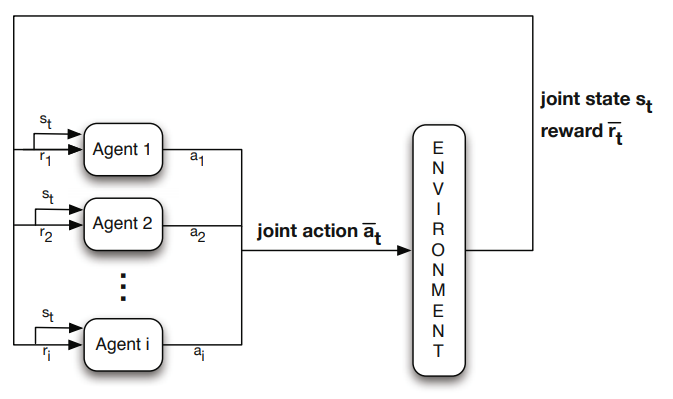
\includegraphics[width=\linewidth]{rlfig}
  \caption{Multiple agents acting in the same environment \cite{rl1}}
  \label{fig:qos}
\end{figure}
%%
An extension of the single agent Markov decision process (MDP) to the multi-agent
case can be defined by Markov Games. In a Markov Game, joint actions are the
result of multiple agents choosing an action independently.
While in normal form games the challenges for reinforcement learners originate
mainly from the interactions between the agents, in Markov games they face the
additional challenge of an environment with state transitions. This means that the
agents typically need to combine coordination methods or equilibrium solvers used
in repeated games with MDP approaches from single-agent RL.
\item  \textbf{Find best delay formula which is the nearest to reality (M/M/1 M/D/1 M/G/1)}


\end{enumerate}

\bibliographystyle{IEEEtran}
\bibliography{references}
\end{document} 